\section{Introduction}\label{sec:introduction}

Polyomino achievement games ask whether one player can obtain a fixed
shape despite an opponent's attempts to obstruct it. In the weak
achievement game, usually called the Maker--Breaker game, only Maker
seeks to complete the shape. The opponent need not make a competing
copy. Snaky is the six-cell target
\begin{equation}\label{eq:target}
 S=\{(0,0),(1,0),(2,0),(3,0),(3,1),(4,1)\}\subset\Z^2.
\end{equation}
Let $\G$ be the eight $2\times2$ signed permutation matrices: each row
and column has one nonzero entry, equal to $1$ or $-1$.
An allowed copy is $t+R(S)$ with $t\in\Z^2$ and $R\in\G$.
Thus reflections and quarter turns are permitted, and scaling is not.
Figure~\ref{fig:target} shows the target in the coordinates of
\eqref{eq:target}.

The board is all of $\Z^2$, initially empty. Maker moves first, and
thereafter Maker and Breaker alternate, each claiming one previously
unclaimed cell. Ownership is permanent. Maker wins immediately upon
owning every cell of an allowed copy, and may own additional cells.
There are no initially owned cells or additional handicap moves.
A strategy chooses a legal cell from the complete finite history.

\begin{theorem}\label{thm:main}
In this game, there is one globally legal Maker policy that completes
an allowed copy of $S$ within at most $21$ actual Maker claims against
every legal continuation of Breaker. Equivalently, extend the policy by
fresh claims after an earlier win: its Maker set after claim $21$
contains a target whenever the first $20$ Breaker replies are legal.
\end{theorem}

The bound counts Maker's actual claims, including any replacement
moves used in the proof. It corresponds to a win no later than the
$41$st individual turn of the alternating game. Corollary~\ref{cor:finite-board}
also gives the same bound on a finite $17\times17$ board. We do not
assert optimal move counts or board sizes, or a result for the strong
game in which both players seek a copy.

\begin{figure}[tb]
\centering
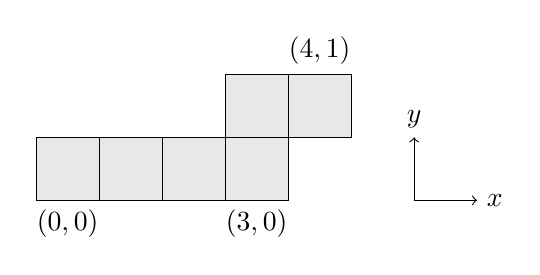
\begin{tikzpicture}[x=8mm,y=8mm]
\foreach \x/\y in {0/0,1/0,2/0,3/0,3/1,4/1}
 {\filldraw[fill=gray!18] (\x,\y) rectangle +(1,1);}
\node[below] at (.5,0) {$(0,0)$};
\node[below] at (3.5,0) {$(3,0)$};
\node[above] at (4.5,2) {$(4,1)$};
\draw[->] (6,0)--(7,0) node[right] {$x$};
\draw[->] (6,0)--(6,1) node[above] {$y$};
\end{tikzpicture}
\caption{The six cells of Snaky. A cell is indexed by the coordinates
of its lower left corner. Every integral translation and signed
coordinate permutation of this shape is an allowed target.}
\label{fig:target}
\end{figure}

\paragraph{Earlier results and methods.}
Sieben attributes the introduction of polyomino achievement games to
Frank Harary \cite[Section~1]{Sieben2004}. His account records
handicap-two strategies of Harary, Harborth and Seemann and the
nonexistence of a pairing defense for Snaky, and proves victory in
$41$ dimensions \cite[Section~4 and Proposition~4.1]{Sieben2004}.
Csernenszky, Martin and Pluh\'ar later gave a computer-free proof of
the nonexistence of a pairing defense
\cite[Theorem~10]{CsernenszkyMartinPluhar2011}.
This rules out a class of Breaker strategies, but does not by itself
give Maker a winning strategy.

Halupczok and Schlage-Puchta proved that Snaky wins in three
dimensions, loses on an $8\times8$ board, and has planar handicap
number at most one \cite[Theorem~1]{HSP2007}.
A handicap of one allows Maker two stones on the opening turn,
before Breaker's first reply.
Ito and Miyagawa also presented a handicap-one construction
\cite{ItoMiyagawa2007}.
Sieben subsequently gave a finite proof sequence for that handicap
and described the ordinary planar problem as undecided at the time
\cite[Section~1 and Appendix~B]{Sieben2008}.

Theorem~\ref{thm:main} treats the empty planar board without a handicap.
We give three complete constructions, with bounds of $21$, $25$, and
$35$ Maker moves. They share a
composition rule but retain different information and different openings.
The $21$-move certificate ends directly with no required Maker stones.
The $25$-move construction removes already-owned cells from each
Breaker-free region and uses required cells as placement anchors.
The $35$-move construction supplies four explicit conditional statements
at arbitrary positions and an opening that reaches one of them.
We keep these methods explicit because their content is not determined by the empty-board
move bounds alone.

Our method belongs to the proof-tree approach to weak achievement
studied by Sieben \cite[Sections~2--3]{Sieben2008}.
His finite situations and territory-intersection conditions encode
ways of combining continuations at Breaker's turn. Our conditional
positions are stated at Maker's turn, with a separate Breaker-turn
consequence for openings in which the pivot is already owned.
The formulation explicitly keeps track of arbitrary previous Maker
and Breaker ownership and counts actual future Maker moves.
We prove its soundness in Section~\ref{sec:templates}.
The perpendicular attacks discussed by Halupczok and Schlage-Puchta
\cite[Section~3]{HSP2007} also illuminate why a line of four Maker
stones can exert substantial pressure. Section~\ref{sec:geometry}
gives a separate, fully stated local result of this kind.

Shaik, Mayer-Eichberger, van de Pol and Saffidine studied bounded-depth
QBF encodings of finite Maker--Breaker games, including Snaky on a
$5\times5$ board \cite[Sections~2.1 and~6]{ShaikEtAl2023}.
Boucher and Villemaire study QBF encodings for finite strong achievement
games on ordinary and toroidal boards
\cite[Sections~2.2, 3.3--3.4, and~4]{BoucherVillemaire2025}.
Here the finite object is a proof of sufficient conditions for the
infinite weak game. Breaker is free to play outside every displayed
region, and the proof covers those replies without a board cutoff.

\paragraph{Proof overview.}
A conditional winning position is described by three finite data:
a set $A$ that Maker must own, a set $T$ that must contain no Breaker
cell, and a bound $h$ on further Maker moves. Starting with the six
immediate completions of $S$, we combine such conditions as follows.
Maker claims a chosen cell. The required cells of every child
condition then belong to Maker; moreover, the intersection of the
child envelopes belongs to Maker. Consequently one new Breaker cell
cannot lie in every child envelope, and at least one continuation
remains available.

Section~\ref{sec:certificate} specifies $728$ numbered conditions,
including the six bases, by exact integer coordinates and backward
references. The final one has $A=\varnothing$, an envelope of $251$
cells, and height $21$. Section~\ref{sec:strategy} turns the recursive
proof into one policy chosen before Breaker's play. The independent
four-in-a-row result follows in Section~\ref{sec:geometry}.
Section~\ref{sec:verification} distinguishes the mathematical induction,
exact data identities, and independent finite calculations.
Appendix~\ref{app:route25} proves the reduced-envelope construction and
its five-class opening. Appendix~\ref{app:route35} gives the complete
$35$-move construction, its unbounded opening, and its conditional tactics.
Appendix~\ref{app:formal} describes the finite reconstruction supplement.
Appendices~\ref{app:data}--\ref{app:data35}
print the three literal certificates, and Appendix~\ref{app:checker}
explains the standalone verification programs.
